\externaldocument{../3/chapter_modeling}
\externaldocument{../4/chapter_algorithm}
\startchapter{Feature Prototype On Atlantis}
\label{chapter:newsol}
In this section I describe the design of the feature prototype of communication identification from the dual\_trace. This prototype is built on top of Atlantis' other features, such as ``memory reconstruction", ``function inspect" and ``views synchronization". Atlantis is an assembly trace analysis environment. It provides many powerful and novel features to assist assembly level execution trace analysis.\cite{huang2017atlantis} This prototype implemented the algorithms described in Chapter\ref{chapter:alo} as well as the user interfaces for the feature.

This prototype consist of three main components: 1) user interface for defining the concerned communication methods' function set. 2) a view that can parallelly present both traces in the dual\_trace. 3) two identification features: Stream identification and communication identification. 4) functionality that allow user to access the identification result.


\section{User Defined Function Set}
As emphasized in Section\ref{windows}, the function set for each communication method can be different depends on the implementation solution of the method. Furthermore, there are so many communication methods in the real world and not all of them are being concerned by the user. Instead of using hard coded function sets, a configuration file in Json format is used for the users to define their concerned communication methods and the corresponding function set. This function sets will be the input for the communication identification. All concerned communication methods have its own function set. The identification features implemented in this prototype iterate all methods in the Json configuration file named ``communicationMethods.json" and identify all communications of each method. This configuration includes the communication method, their function set for the communication events and the essential parameters of each function. A default template is given for user reference, this default template is generated by Atlantis when it was launched and stored in the .tmp folder in the trace analysis project folder. Only Named pipe as a communication method is listed in this template. User can change this file to add or remove their concerned communication methods. The default template example can be find in Section\ref{funcset}.

\section{Parallel Editor View For Dual\_Trace}
The dual\_trace consist of two execution traces which are interacting with each other. To present them in the same view makes the analysis for the user much easier. The strategy to open parallel editor view is that open one trace as the normal one and the other as the dual\_trace of the current opened one. A new menu option in the project navigation view are created for opening the second trace as the dual\_trace for the current active trace editor. The implementation of the parallel editor take the advantage of the existing SWT of Eclipse plug-in development. The detail of the implementation can be found in Section\ref{paralleleditor}. Figure\ref{opendualtracemenu} shows this menu option and Figure\ref{paralleleditor}.

\begin{figure}[H]
\centerline{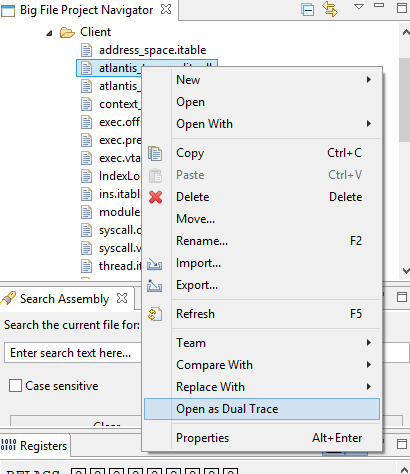
\includegraphics[scale=0.48]{Figures/opendualtracemenu}}
 \caption{Menu Item for opening Dual\_trace}
\label{opendualtracemenu}
\end{figure}

\begin{figure}[H]
\centerline{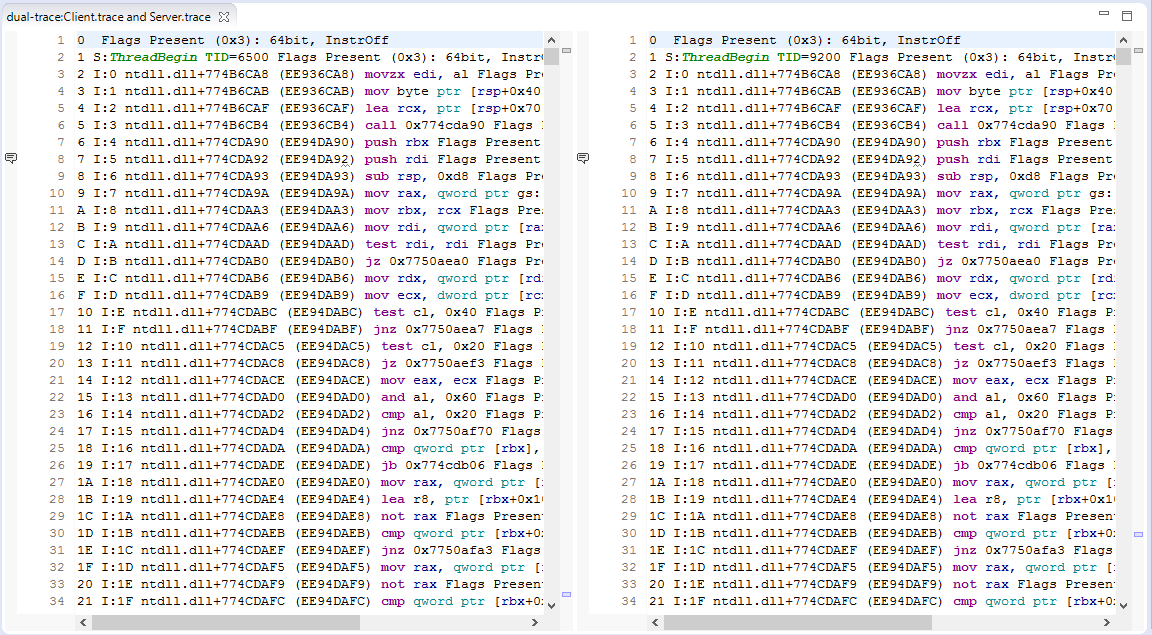
\includegraphics[scale=0.48]{Figures/paralleleditor}}
 \caption{Parallel Editor View}
\label{paralleleditor}
\end{figure}



\section{Identification Features}
I implemented two identification features, one is stream identification for both traces in the dual\_trace, the other is the communication identification. These two features align to the ``stream identification algorithm" and ``communication identification algorithm" designed in Chapter\ref{chapter:alo}. The implementation the identification features relies on the existing ``function inspect" feature of Atlantis. The called functions' name can be inspected  by  search of the symbolic name in the executable binary or any DLLs which used by the program at the time when it is traced. By importing the DLLs and execution  executable binary, Atlantis can recognize the function call from the execution trace by the function names. A new menu ``Dual\_trace Tool" with two menu options ``Stream Identification" and ``Communication Identification" are designed for these two identification features. Figure\ref{opendualtracemenu} shows this new menu in Atlantis. A new  ``Communication" view is designed for presenting the identification of the streams and communication. There are two sub tables in this view, the right one is for the stream identification result while the left one is for communication identification result. The reason for putting this two result in the same view is for easy access and comparison of the data for the users. Figure\ref{opendualtracemenu} shows this view with result data in it. each time when the user rerun the identification feature the result in the corresponding table will be refreshed to show only the latest identification result. But the other table will not be affected and its own last identification result will stay. For example, if the user run the ``Stream Identification" feature first, the stream identification result will show on the left table of the view. And then the user run the ``communication Identification", the communication identification result will be shown on the right table while the left one still holding the last stream identification result.


\section{Identification Result View and Result Navigation}
To allow the user 


